\chapter{Исследовательская часть}

В данном разделе будут приведены примеры работы программы, и будет проведен сравнительный анализ реализованных алгоритмов по числу строк и по длине строк.

\section{Технические характеристики}

Тестирование проводилось на устройстве со следующими техническими характеристиками:

\begin{itemize}
	\item операционная система: Ubuntu 20.04.1 Linux x86\_64 \cite{linux};
	\item память : 8 GiB;
	\item процессор: AMD® Ryzen™ 3 3200u @ 2.6 GHz;
	\item 4 физических ядра, 4 логических ядра \cite{amd}.
\end{itemize}

Тестирование проводилось на ноутбуке, включенном в сеть электропитания. Во время тестирования ноутбук был нагружен только встроенными приложениями окружения, а также непосредственно системой тестирования.

\clearpage

\section{Демонстрация работы программы}

На рисунке \ref{img:example-linear} приведен пример последовательной обработки, на рисунке \ref{img:example-parallel} - пример конвейерной обработки.

\begin{figure}[H]
	\begin{center}
		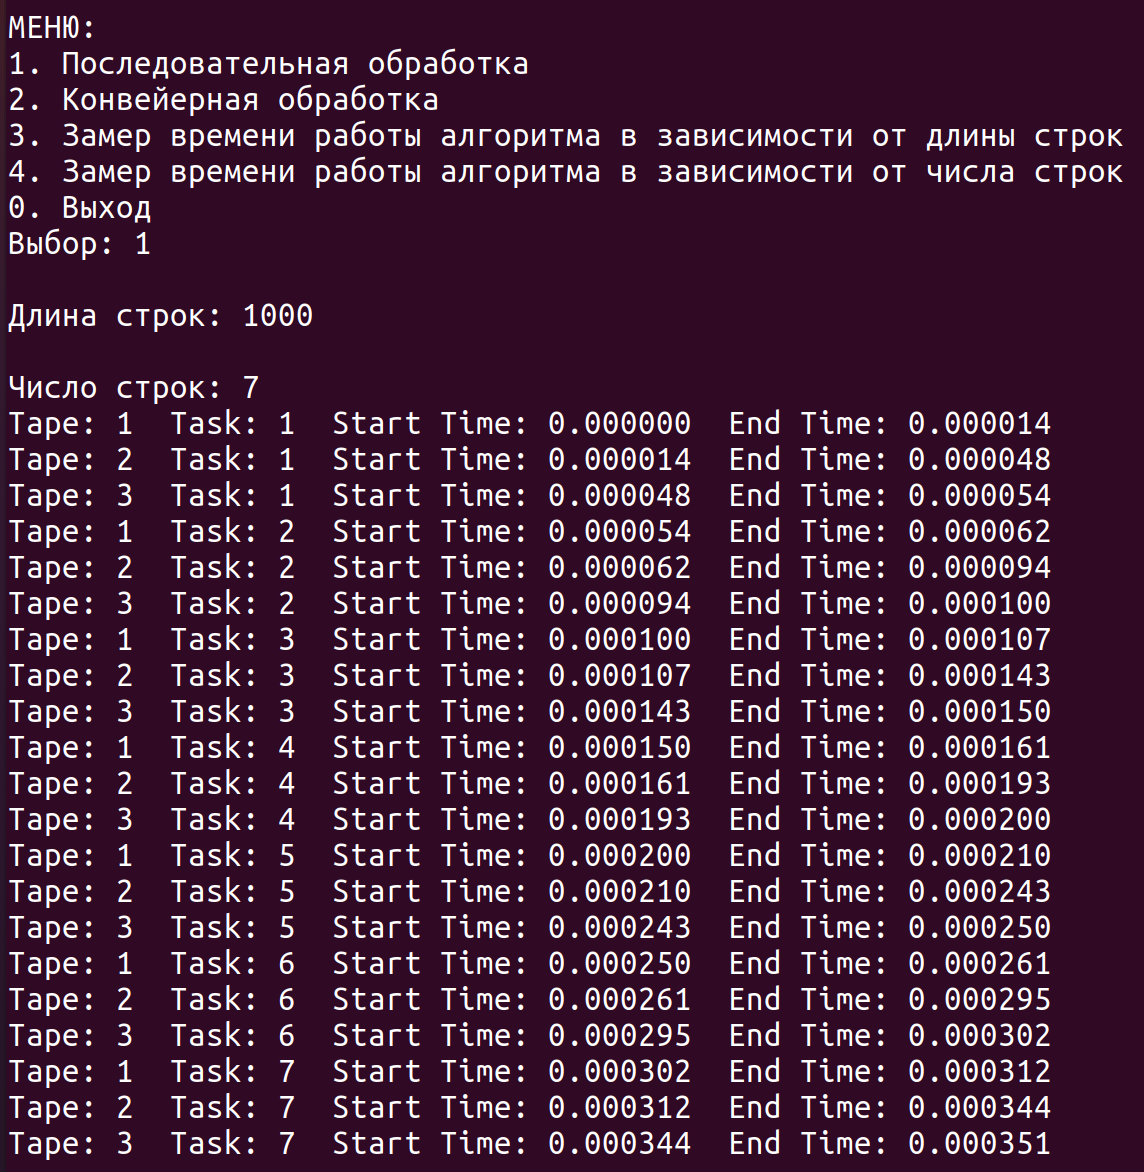
\includegraphics[scale=0.3]{img/example-linear.png}
	\end{center}
	\captionsetup{justification=centering}
	\caption{Пример последовательной обработки}
	\label{img:example-linear}
\end{figure}

\begin{figure}[H]
	\begin{center}
		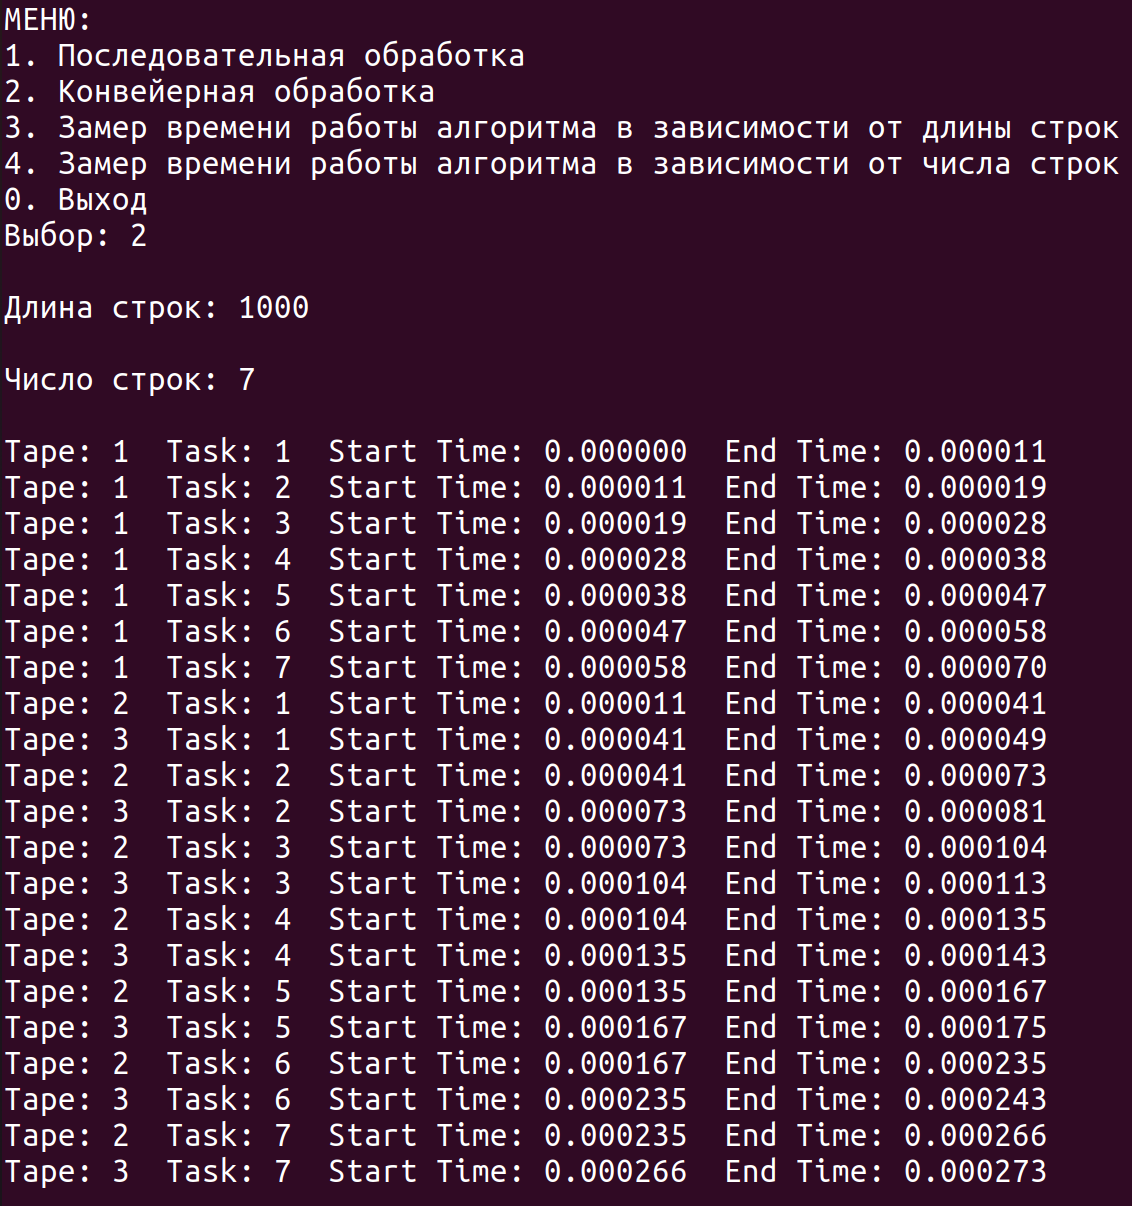
\includegraphics[scale=0.3]{img/example-parallel.png}
	\end{center}
	\captionsetup{justification=centering}
	\caption{Пример конвейерной обработки}
	\label{img:example-parallel}
\end{figure}

\section{Время выполнения алгоритмов}

Функция $std::chrono::system\_clock::now(...)$ из библиотеки $chrono$ ЯП $C++$ возвращает  процессорное время в секундах - значение типа float.

Для замера времени необходимо получить значение времени до начала выполнения алгоритма, затем после его окончания. Чтобы получить результат, необходимо вычесть из второго значения первое.

Сравнительный анализ по времени в зависимости от числа строк проводился для строк-палиндромов, заполненных случайным образом, длиной 6000 символов. Результаты измерения времени приведены в таблице \ref{tbl:time_count_str} (в с).

\begin{table}[h]
    \begin{center}
        \begin{threeparttable}
        \captionsetup{justification=raggedright,singlelinecheck=off}
        \caption{Результаты замеров времени в зависимости от числа строк}
        \label{tbl:time_count_str}
        \begin{tabular}{|c|c|c|c|}
            \hline
            Число строк & Конвейерная & Последовательная \\
            \hline
            10 & 0.00150191 & 0.00208726 \\ \hline  
            20 & 0.0026085 & 0.00298096 \\ \hline
            30 & 0.00288755 & 0.00376455 \\ \hline
            40 & 0.00439648 & 0.0047981  \\ \hline 
            50 & 0.00562291 & 0.00612586 \\ \hline
		\end{tabular}
    \end{threeparttable}
\end{center}
\end{table}

На рисунке \ref{img:count_str} приведены графические результаты сравнения временных характеристик для различного числа потоков.

\begin{figure}[H]
	\begin{center}
		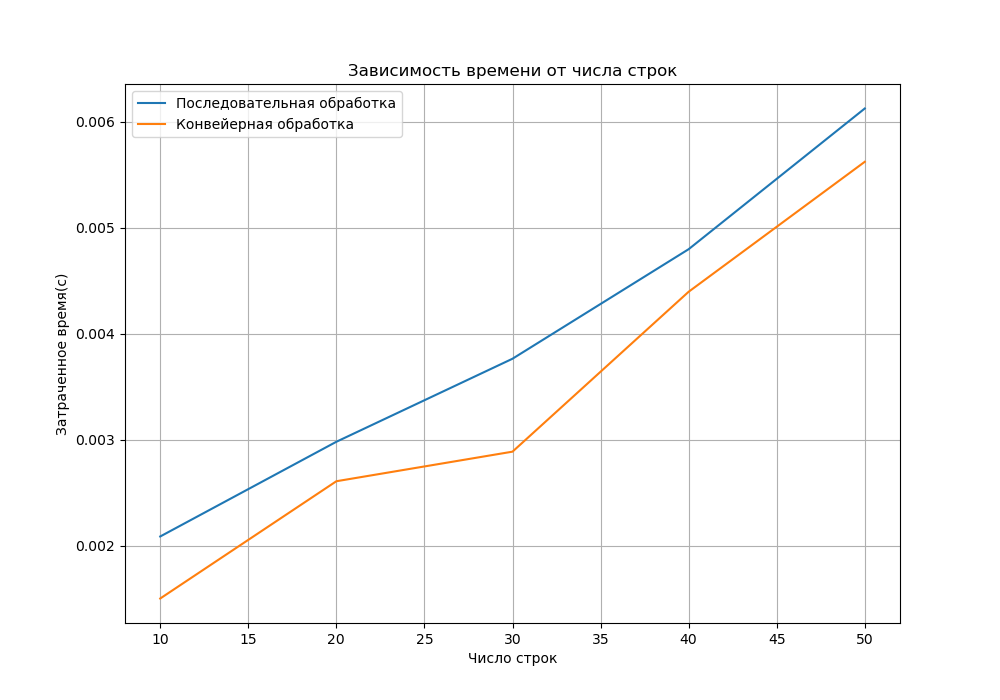
\includegraphics[scale=0.5]{img/count_str.png}
	\end{center}
	\captionsetup{justification=centering}
	\caption{Сравнение по времени в зависимости от числа строк}
	\label{img:count_str}
\end{figure}

Кроме того, замеры времени проводились для строк-палиндромов, заполненных случайным образом, длиной от 10000 до 100000 символов с шагом в 10000 символов. Результаты измерения времени в зависимости от длины строк приведены в таблице \ref{tbl:time_len} (в с).

\begin{table}[h]
    \begin{center}
        \begin{threeparttable}
        \captionsetup{justification=raggedright,singlelinecheck=off}
        \caption{Результаты замеров времени в зависимости от порядка графа}
        \label{tbl:time_len}
        \begin{tabular}{|c|c|c|c|}
            \hline
            Число строк & Конвейерная & Последовательная \\
            \hline
            10000 & 0.00353928 & 0.00423032 \\ \hline  
            20000 & 0.00321933 & 0.00492197 \\ \hline
            30000 & 0.00478432 & 0.00982671 \\ \hline
            40000 & 0.0114914 & 0.0148205  \\ \hline 
            50000 & 0.0132036 & 0.0195122 \\ \hline
            60000 & 0.0230261 & 0.0263445 \\ \hline
            70000 & 0.0223084 & 0.0308759 \\ \hline
            80000 & 0.0344795 & 0.0368916 \\ \hline
            90000 & 0.0372315 & 0.0488796 \\ \hline
            100000 & 0.0499187 & 0.0527271 \\ \hline                                           
		\end{tabular}
    \end{threeparttable}
\end{center}
\end{table}

На рисунке \ref{img:len} приведены графические результаты сравнения временных характеристик для различной длины строк.

\begin{figure}[H]
	\begin{center}
		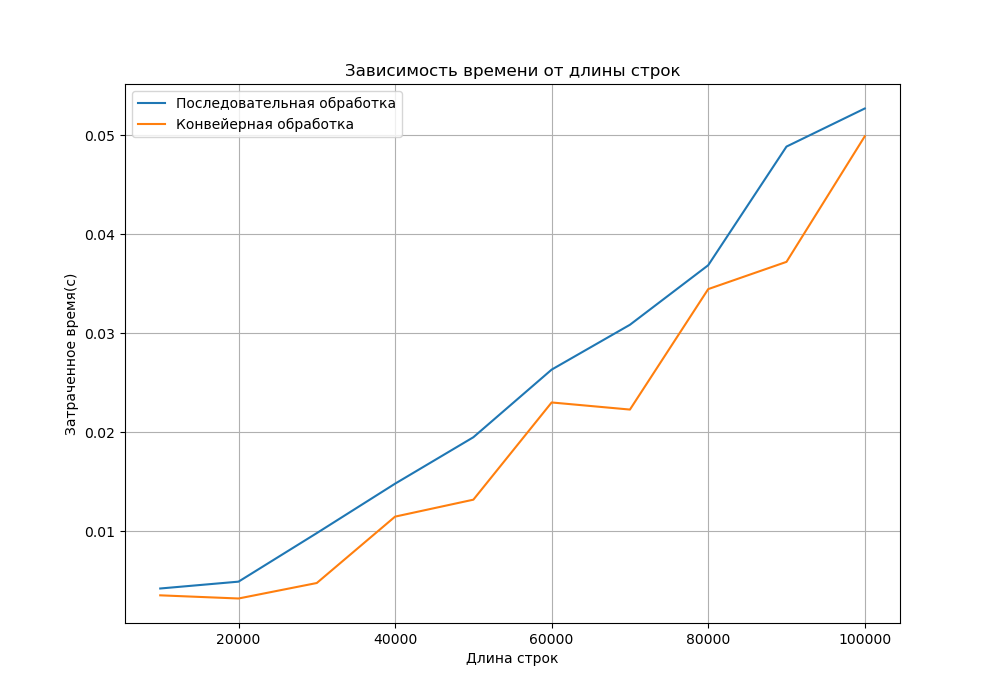
\includegraphics[scale=0.5]{img/len.png}
	\end{center}
	\captionsetup{justification=centering}
	\caption{Сравнение по времени в зависимости от длины строк}
	\label{img:len}
\end{figure}

\section{Вывод}

В результате эксперимента было получено, что конвейерная обработка 30 строк в 1.3 раза быстрее последовательной обработки строк-палиндромов длиной 6000 символов. Тогда, для указанных данных небходимо использовать конвейерную обработку данных.

Также в результате сравнительного анализа было установлено, что при увеличении длины строк конвейерная обработка быстрее последовательной: при длине, равной 20000 символам - в 1.5 раза, при длине, равной 30000 - в 2 раза. Можно сделать вывод, что конвейерную обработку следует применять при больших значениях длины строк.